% ==================================================
% CHAPTER 5: Using x-rays to measure relative strip position offsets
% ==================================================

\chapter{Using x-rays to measure relative strip position offsets}
\label{chap:xray}

%TODO : consistently call the x-ray centroids the "x-ray beam profile centers"

Other work on characterizing relative alignments between quadruplet layers has been completed~\cite{zhao_cosmic_2019} or is ongoing, \textcolor{red}{(Can I cite John's thesis-in-progress?)} but what is required are the absolute strip positions with respect to their nominal position in the ATLAS analysis coordinate system to be input into \package{Athena}~\cite{the_atlas_collaboration_athena}. Somehow, alignment parameters must be derived to create a model of absolute strip positions - which is not possible with the cosmics dataset. Absolute local offset measurements were done by the so-called x-ray method. The author did not partake in the design of or data collection with this method. The reader is referred to the paper~\cite{lefebvre_precision_2020}, describing the x-ray method.

% --------------------------------------------------
\section{Experimental setup}
% --------------------------------------------------

The x-ray tests were performed after the quadruplets arrived at CERN, were assembled into wedges, and alignment platforms installed. Essentially, an x-ray gun was attached to one of the alignment platforms glued to the surface of the wedge and the beam profile recorded by the strips.

\begin{figure}
    \centering
    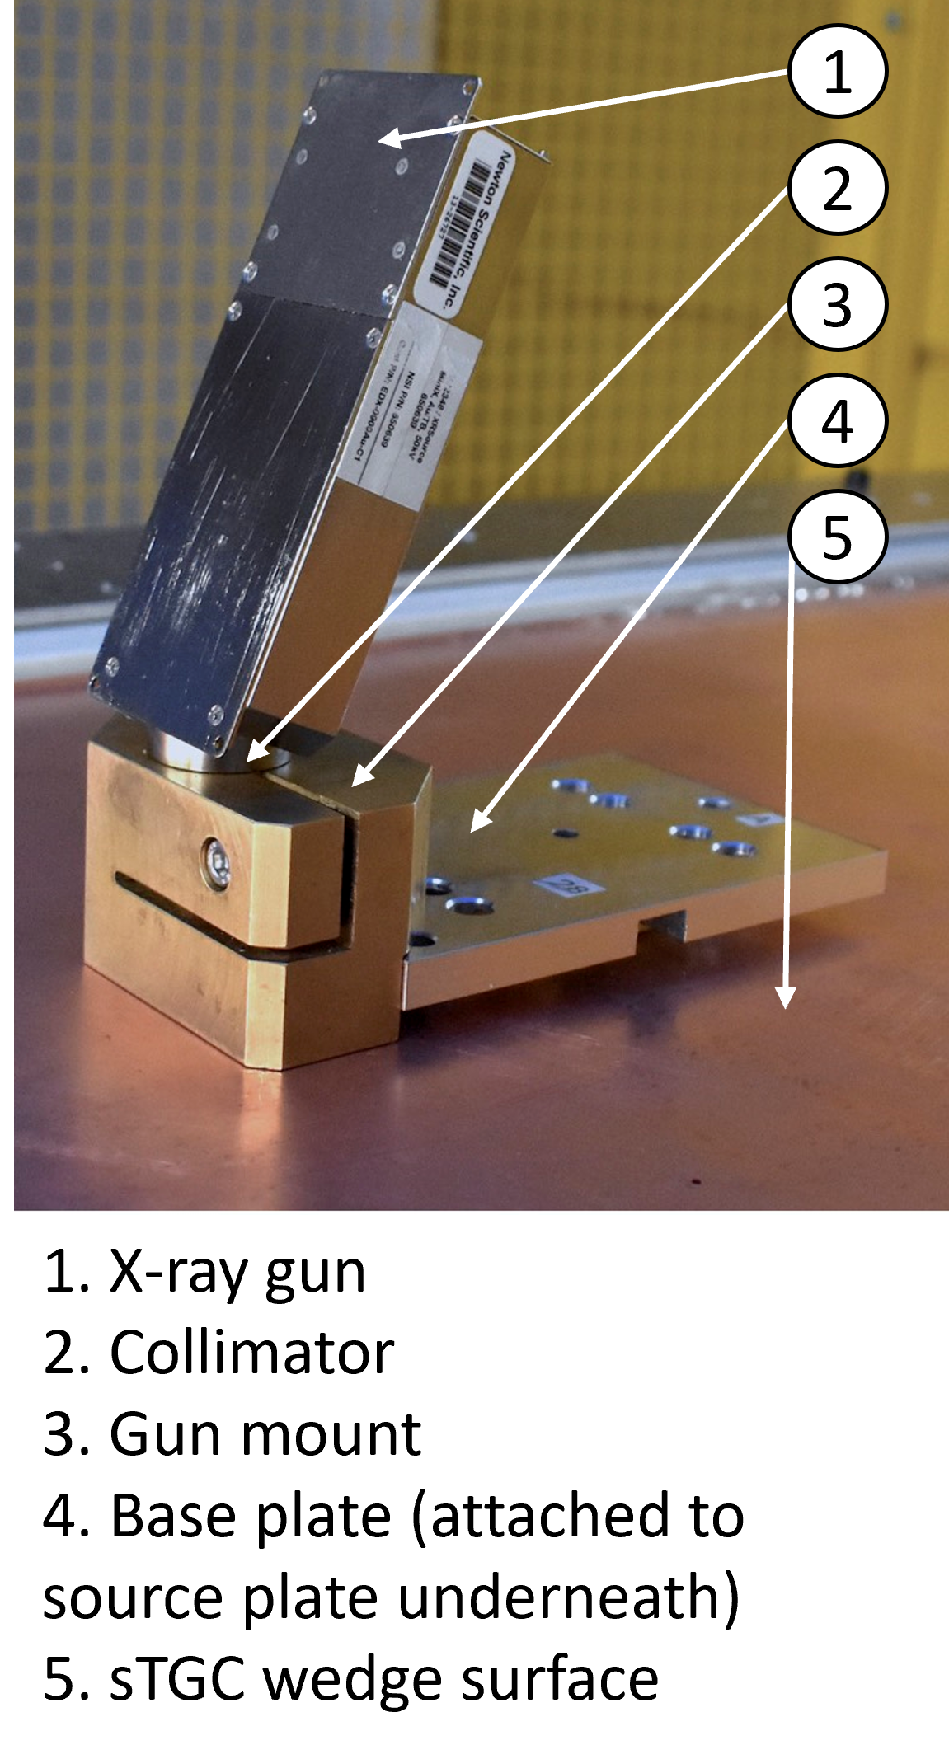
\includegraphics[width = 0.5\textwidth]{figures/figure_xray_setup.pdf}
    \caption{The x-ray gun mounted to the alignment platform on the surface of the wedge. Adapted from~\cite{lefebvre_precision_2020}.}
    \label{fig:xray_setup}
\end{figure}

The wedges were installed on carts that could rotate their surface to a horizontal position. A mounting platform was installed on top of the alignment platform using a three-ball mount. The x-ray gun used was an \href{https://www.amptek.com/-/media/ametekamptek/documents/resources/specs/mini-x-specifications.pdf?la=en\&revision=512f7eb3-01b3-47fd-864f-5525c850fc6e\&hash=B8B03C0592486E2D91C566C4326F15F5}{Amptek Mini-X tube}. The gun was placed in a brass holder with built-in \SI{2}{mm} collimator and \SI{280}{\micro\meter} copper filter that be mounted on one of five positions on the mounting platform, as shown in figure~\ref{fig:xray_setup}. Gun positions were chosen to avoid wire support structures in the sTGCs that reduce hit efficiency~\cite{lefebvre_thesis} and boundaries between sets of strips readout by two different ASICs (each ASIC had 64 channels that could be connected to electrodes) that could each have different thresholds. 

As with cosmics data collection, each sTGC also needed gas and high voltage to operate. Each layer was operated at \SI{2.925}{kV} with high voltage from a NIM crate. The chambers were flushed with CO$_2$ before and during data collection.

% During ATLAS operation, the position of the source plates will be monitored using the new alignment system~\cite{nsw_tdr}. Therefore, their position will be known in the absolute ATLAS coordinate system. 

% --------------------------------------------------
\section{Data acquisition}
% --------------------------------------------------

A different version of the same front end electronics used in cosmics testing were used for the x-ray testing. Data was collected for two minutes per gun position with random triggers. The gun produced x-rays under \SI{50}{\kilo\electronvolt}. Peaks in the 0-\SI{30}{keV} range were filtered out by the copper filter and the copper of the sTGCs. The copper filter helped to reduce the effect of attenuation non-uniformities. The x-rays mostly interacted with the wedge's copper electrodes and gold-plated tungsten wires via the photo effect. The resulting photoelectrons caused ionization avalanches. The beam profile was captured by the distribution of cluster positions. A typical beam profile is shown in figure~\ref{fig:xray_beam_profile}.

\begin{figure}
    \centering
    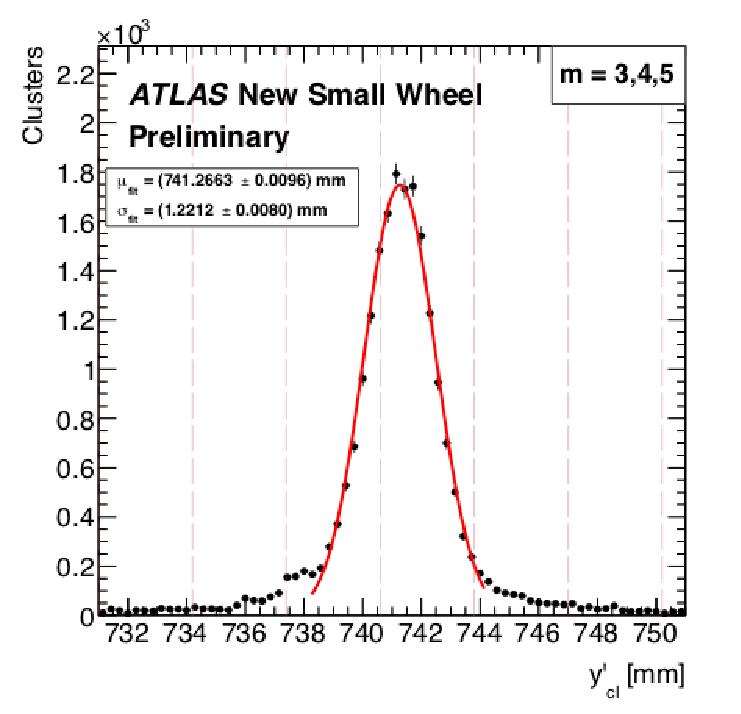
\includegraphics[width = 0.5\textwidth]{figures/figure_xray_beam_profile.pdf}
    \caption{Distribution of x-ray cluster mean positions after the analysis cuts and corrections. The strip cluster multiplicity, $m$, was limited to 3, 4 and 5. The red line is a Gaussian fit of the distribution and the pink lines denote the edges of the strips. Adapted from \copyright CERN for the benefit of the ATLAS collaboration. CC-BY-4.0 license.}
    \label{fig:xray_beam_profile}
\end{figure}

% --------------------------------------------------
\section{Data preparation}
% --------------------------------------------------
YOU ARE HERE
Clusters with signal on more than 5 strips were cut because they were most likely caused by photoelectrons ejected with enough energy to cause more primary ionization and subsequent avalanches ($\delta$-rays)~\cite{lefebvre_precision_2020}.

The mean of the cluster position distribution was taken as the x-ray beam profile center. The expected center was calculated assuming a wedge with nominal geometry given the gun position. The difference between the expected and reconstructed beam profile center is a measure of the local offset. Applying the logic of equation~\ref{eqn:local_translation} to the beam profile, the fitted mean acts as $y$, the expected center is $y_{nom}$ and the local offset is $d_{local}$ as before. The x-ray local offsets  give the absolute local position of the strip pattern with respect to the source plates. Since the position of the source plates will be monitored by the alignment system in ATLAS~\cite{nsw_tdr}, the local position of the strip pattern can be known in the ATLAS coordinate system for every position where x-ray data was taken.

%TODO : Maybe move this paragraph to start of comparison chapter
The main advantage of the x-ray dataset over the cosmics dataset is that absolute local offsets are measurable thanks to the reference frame provided by the source plates. However, the systematic uncertainty on the x-ray offsets is large: \SI{120}{\micro\meter} was accepted by the collaboration. The cuts and corrections applied to the x-ray data that motivate the uncertainty are detailed in Lefebvre, 2020~\cite{lefebvre_precision_2020}. In addition, local offset measurements were limited to the positions of the alignment platforms; only 10 - 20 positions were surveyed for each wedge. Therefore, validating the x-ray measurements and seeing how they can be improved is important because of the uncertainty in and incompleteness of the dataset. How the cosmics dataset was used for this purpose is discussed in chapter~\ref{chap:comparison}. 